% Options for packages loaded elsewhere
\PassOptionsToPackage{unicode}{hyperref}
\PassOptionsToPackage{hyphens}{url}
%
\documentclass[
]{article}
\usepackage{amsmath,amssymb}
\usepackage{iftex}
\ifPDFTeX
  \usepackage[T1]{fontenc}
  \usepackage[utf8]{inputenc}
  \usepackage{textcomp} % provide euro and other symbols
\else % if luatex or xetex
  \usepackage{unicode-math} % this also loads fontspec
  \defaultfontfeatures{Scale=MatchLowercase}
  \defaultfontfeatures[\rmfamily]{Ligatures=TeX,Scale=1}
\fi
\usepackage{lmodern}
\ifPDFTeX\else
  % xetex/luatex font selection
\fi
% Use upquote if available, for straight quotes in verbatim environments
\IfFileExists{upquote.sty}{\usepackage{upquote}}{}
\IfFileExists{microtype.sty}{% use microtype if available
  \usepackage[]{microtype}
  \UseMicrotypeSet[protrusion]{basicmath} % disable protrusion for tt fonts
}{}
\makeatletter
\@ifundefined{KOMAClassName}{% if non-KOMA class
  \IfFileExists{parskip.sty}{%
    \usepackage{parskip}
  }{% else
    \setlength{\parindent}{0pt}
    \setlength{\parskip}{6pt plus 2pt minus 1pt}}
}{% if KOMA class
  \KOMAoptions{parskip=half}}
\makeatother
\usepackage{xcolor}
\usepackage[margin=1in]{geometry}
\usepackage{color}
\usepackage{fancyvrb}
\newcommand{\VerbBar}{|}
\newcommand{\VERB}{\Verb[commandchars=\\\{\}]}
\DefineVerbatimEnvironment{Highlighting}{Verbatim}{commandchars=\\\{\}}
% Add ',fontsize=\small' for more characters per line
\usepackage{framed}
\definecolor{shadecolor}{RGB}{248,248,248}
\newenvironment{Shaded}{\begin{snugshade}}{\end{snugshade}}
\newcommand{\AlertTok}[1]{\textcolor[rgb]{0.94,0.16,0.16}{#1}}
\newcommand{\AnnotationTok}[1]{\textcolor[rgb]{0.56,0.35,0.01}{\textbf{\textit{#1}}}}
\newcommand{\AttributeTok}[1]{\textcolor[rgb]{0.13,0.29,0.53}{#1}}
\newcommand{\BaseNTok}[1]{\textcolor[rgb]{0.00,0.00,0.81}{#1}}
\newcommand{\BuiltInTok}[1]{#1}
\newcommand{\CharTok}[1]{\textcolor[rgb]{0.31,0.60,0.02}{#1}}
\newcommand{\CommentTok}[1]{\textcolor[rgb]{0.56,0.35,0.01}{\textit{#1}}}
\newcommand{\CommentVarTok}[1]{\textcolor[rgb]{0.56,0.35,0.01}{\textbf{\textit{#1}}}}
\newcommand{\ConstantTok}[1]{\textcolor[rgb]{0.56,0.35,0.01}{#1}}
\newcommand{\ControlFlowTok}[1]{\textcolor[rgb]{0.13,0.29,0.53}{\textbf{#1}}}
\newcommand{\DataTypeTok}[1]{\textcolor[rgb]{0.13,0.29,0.53}{#1}}
\newcommand{\DecValTok}[1]{\textcolor[rgb]{0.00,0.00,0.81}{#1}}
\newcommand{\DocumentationTok}[1]{\textcolor[rgb]{0.56,0.35,0.01}{\textbf{\textit{#1}}}}
\newcommand{\ErrorTok}[1]{\textcolor[rgb]{0.64,0.00,0.00}{\textbf{#1}}}
\newcommand{\ExtensionTok}[1]{#1}
\newcommand{\FloatTok}[1]{\textcolor[rgb]{0.00,0.00,0.81}{#1}}
\newcommand{\FunctionTok}[1]{\textcolor[rgb]{0.13,0.29,0.53}{\textbf{#1}}}
\newcommand{\ImportTok}[1]{#1}
\newcommand{\InformationTok}[1]{\textcolor[rgb]{0.56,0.35,0.01}{\textbf{\textit{#1}}}}
\newcommand{\KeywordTok}[1]{\textcolor[rgb]{0.13,0.29,0.53}{\textbf{#1}}}
\newcommand{\NormalTok}[1]{#1}
\newcommand{\OperatorTok}[1]{\textcolor[rgb]{0.81,0.36,0.00}{\textbf{#1}}}
\newcommand{\OtherTok}[1]{\textcolor[rgb]{0.56,0.35,0.01}{#1}}
\newcommand{\PreprocessorTok}[1]{\textcolor[rgb]{0.56,0.35,0.01}{\textit{#1}}}
\newcommand{\RegionMarkerTok}[1]{#1}
\newcommand{\SpecialCharTok}[1]{\textcolor[rgb]{0.81,0.36,0.00}{\textbf{#1}}}
\newcommand{\SpecialStringTok}[1]{\textcolor[rgb]{0.31,0.60,0.02}{#1}}
\newcommand{\StringTok}[1]{\textcolor[rgb]{0.31,0.60,0.02}{#1}}
\newcommand{\VariableTok}[1]{\textcolor[rgb]{0.00,0.00,0.00}{#1}}
\newcommand{\VerbatimStringTok}[1]{\textcolor[rgb]{0.31,0.60,0.02}{#1}}
\newcommand{\WarningTok}[1]{\textcolor[rgb]{0.56,0.35,0.01}{\textbf{\textit{#1}}}}
\usepackage{graphicx}
\makeatletter
\def\maxwidth{\ifdim\Gin@nat@width>\linewidth\linewidth\else\Gin@nat@width\fi}
\def\maxheight{\ifdim\Gin@nat@height>\textheight\textheight\else\Gin@nat@height\fi}
\makeatother
% Scale images if necessary, so that they will not overflow the page
% margins by default, and it is still possible to overwrite the defaults
% using explicit options in \includegraphics[width, height, ...]{}
\setkeys{Gin}{width=\maxwidth,height=\maxheight,keepaspectratio}
% Set default figure placement to htbp
\makeatletter
\def\fps@figure{htbp}
\makeatother
\setlength{\emergencystretch}{3em} % prevent overfull lines
\providecommand{\tightlist}{%
  \setlength{\itemsep}{0pt}\setlength{\parskip}{0pt}}
\setcounter{secnumdepth}{-\maxdimen} % remove section numbering
\ifLuaTeX
  \usepackage{selnolig}  % disable illegal ligatures
\fi
\usepackage{bookmark}
\IfFileExists{xurl.sty}{\usepackage{xurl}}{} % add URL line breaks if available
\urlstyle{same}
\hypersetup{
  pdftitle={st440hw5r},
  pdfauthor={Logan Moy},
  hidelinks,
  pdfcreator={LaTeX via pandoc}}

\title{st440hw5r}
\author{Logan Moy}
\date{2025-03-19}

\begin{document}
\maketitle

\subsection{Jags}\label{jags}

\subsection{3.9}\label{section}

\begin{Shaded}
\begin{Highlighting}[]
  \CommentTok{\# Y is num of home runs}
\NormalTok{  data }\OtherTok{\textless{}{-}} \FunctionTok{list}\NormalTok{(}\AttributeTok{regY =} \DecValTok{563}\NormalTok{, }\AttributeTok{regN =} \DecValTok{2820}\NormalTok{, }\AttributeTok{worldY =} \DecValTok{10}\NormalTok{, }\AttributeTok{worldN =} \DecValTok{27}\NormalTok{)}

\NormalTok{  model\_string }\OtherTok{\textless{}{-}} \FunctionTok{textConnection}\NormalTok{(}\StringTok{"model\{}

\StringTok{   \# Likelihood}
\StringTok{    regY \textasciitilde{} dpois(regN * lambda1)}
\StringTok{    worldY \textasciitilde{} dpois(worldN * lambda2)}

\StringTok{   \# Priors}
\StringTok{    lambda1 \textasciitilde{}  dunif(0, 10)}
\StringTok{    lambda2 \textasciitilde{}  dunif(0, 10)}
\StringTok{    ratio \textless{}{-} lambda2/lambda1}
\StringTok{ \}"}\NormalTok{)}

\NormalTok{ inits }\OtherTok{\textless{}{-}} \FunctionTok{list}\NormalTok{(}\AttributeTok{lambda1 =} \FloatTok{0.1}\NormalTok{,}\AttributeTok{lambda2 =} \FloatTok{0.1}\NormalTok{)}
\NormalTok{ model }\OtherTok{\textless{}{-}} \FunctionTok{jags.model}\NormalTok{(model\_string, }\AttributeTok{data =}\NormalTok{ data, }\AttributeTok{inits=}\NormalTok{inits, }\AttributeTok{n.chains=}\DecValTok{2}\NormalTok{, }\AttributeTok{quiet=}\ConstantTok{TRUE}\NormalTok{)}
 \FunctionTok{update}\NormalTok{(model, }\DecValTok{10000}\NormalTok{, }\AttributeTok{progress.bar=} \StringTok{"none"}\NormalTok{)}
\NormalTok{ params  }\OtherTok{\textless{}{-}} \FunctionTok{c}\NormalTok{(}\StringTok{"lambda1"}\NormalTok{,}\StringTok{"lambda2"}\NormalTok{,}\StringTok{"ratio"}\NormalTok{)}
 
\NormalTok{ samples }\OtherTok{\textless{}{-}} \FunctionTok{coda.samples}\NormalTok{(model, }
            \AttributeTok{variable.names=}\NormalTok{params, }
            \AttributeTok{n.iter=}\DecValTok{10000}\NormalTok{, }\AttributeTok{progress.bar=} \StringTok{"none"}\NormalTok{)}

 
 \FunctionTok{plot}\NormalTok{(samples)}
\end{Highlighting}
\end{Shaded}

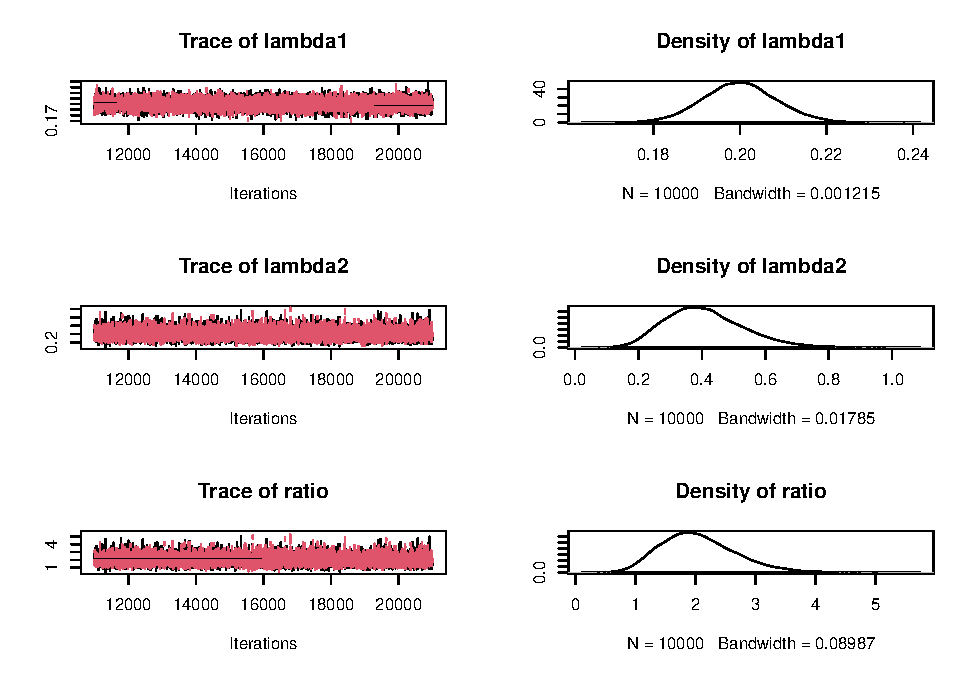
\includegraphics{st440hw5_files/figure-latex/unnamed-chunk-1-1.pdf}

\begin{Shaded}
\begin{Highlighting}[]
 \FunctionTok{summary}\NormalTok{(samples)}
\end{Highlighting}
\end{Shaded}

\begin{verbatim}
## 
## Iterations = 11001:21000
## Thinning interval = 1 
## Number of chains = 2 
## Sample size per chain = 10000 
## 
## 1. Empirical mean and standard deviation for each variable,
##    plus standard error of the mean:
## 
##           Mean       SD  Naive SE Time-series SE
## lambda1 0.2000 0.008408 5.946e-05      7.784e-05
## lambda2 0.4096 0.123013 8.698e-04      1.189e-03
## ratio   2.0513 0.622080 4.399e-03      6.118e-03
## 
## 2. Quantiles for each variable:
## 
##           2.5%    25%    50%    75%  97.5%
## lambda1 0.1837 0.1944 0.1999 0.2055 0.2169
## lambda2 0.2061 0.3215 0.3978 0.4851 0.6802
## ratio   1.0285 1.6067 1.9898 2.4301 3.4347
\end{verbatim}

\begin{Shaded}
\begin{Highlighting}[]
 \FunctionTok{effectiveSize}\NormalTok{(samples)}
\end{Highlighting}
\end{Shaded}

\begin{verbatim}
##  lambda1  lambda2    ratio 
## 11692.92 10702.54 10367.52
\end{verbatim}

\begin{Shaded}
\begin{Highlighting}[]
 \FunctionTok{gelman.diag}\NormalTok{(samples)}
\end{Highlighting}
\end{Shaded}

\begin{verbatim}
## Potential scale reduction factors:
## 
##         Point est. Upper C.I.
## lambda1          1          1
## lambda2          1          1
## ratio            1          1
## 
## Multivariate psrf
## 
## 1
\end{verbatim}

Convergence: The Gel statistic are all exactly 1 and the effective
sample sizes are also large (10K+). The trace plots also look good with
a ``barcode'' shape and don't converge to a single point. All of this
points to converging chains.

\subsection{4.1}\label{section-1}

\begin{Shaded}
\begin{Highlighting}[]
  \CommentTok{\# Setting up data for jags}
\NormalTok{  nplace }\OtherTok{\textless{}{-}}\NormalTok{ ntreat }\OtherTok{\textless{}{-}} \DecValTok{6}
\NormalTok{  placebo }\OtherTok{\textless{}{-}} \FunctionTok{c}\NormalTok{(}\FloatTok{2.0}\NormalTok{, }\SpecialCharTok{{-}}\FloatTok{3.1}\NormalTok{, }\SpecialCharTok{{-}}\FloatTok{1.0}\NormalTok{, }\FloatTok{0.2}\NormalTok{, }\FloatTok{0.3}\NormalTok{, }\FloatTok{0.4}\NormalTok{)}
\NormalTok{  treat    }\OtherTok{\textless{}{-}} \FunctionTok{c}\NormalTok{(}\SpecialCharTok{{-}}\FloatTok{3.5}\NormalTok{, }\SpecialCharTok{{-}}\FloatTok{1.6}\NormalTok{, }\SpecialCharTok{{-}}\FloatTok{4.6}\NormalTok{, }\SpecialCharTok{{-}}\FloatTok{0.9}\NormalTok{, }\SpecialCharTok{{-}}\FloatTok{5.1}\NormalTok{, }\FloatTok{0.1}\NormalTok{)}
   
\NormalTok{  meanplacebo }\OtherTok{\textless{}{-}} \FunctionTok{mean}\NormalTok{(placebo)}
\NormalTok{  meantreat }\OtherTok{\textless{}{-}} \FunctionTok{mean}\NormalTok{(treat)}
  
\NormalTok{  s2pl   }\OtherTok{\textless{}{-}} \FunctionTok{mean}\NormalTok{((placebo }\SpecialCharTok{{-}}\NormalTok{ meanplacebo)}\SpecialCharTok{\^{}}\DecValTok{2}\NormalTok{)}
\NormalTok{  s2trt   }\OtherTok{\textless{}{-}} \FunctionTok{mean}\NormalTok{((treat }\SpecialCharTok{{-}}\NormalTok{ meantreat)}\SpecialCharTok{\^{}}\DecValTok{2}\NormalTok{)}
\NormalTok{  sp    }\OtherTok{\textless{}{-}} \FunctionTok{sqrt}\NormalTok{((s2pl}\SpecialCharTok{/}\DecValTok{2} \SpecialCharTok{+}\NormalTok{ s2trt}\SpecialCharTok{/}\DecValTok{2}\NormalTok{))}

\NormalTok{  postmean }\OtherTok{\textless{}{-}}\NormalTok{ meantreat }\SpecialCharTok{{-}}\NormalTok{ meanplacebo}
\NormalTok{  postsd }\OtherTok{\textless{}{-}}\NormalTok{ sp }\SpecialCharTok{*} \FunctionTok{sqrt}\NormalTok{( }\DecValTok{1}\SpecialCharTok{/}\NormalTok{nplace }\SpecialCharTok{+} \DecValTok{1}\SpecialCharTok{/}\NormalTok{ntreat)}
\NormalTok{  credset }\OtherTok{\textless{}{-}}\NormalTok{ postmean }\SpecialCharTok{+}\NormalTok{ postsd }\SpecialCharTok{*} \FunctionTok{qt}\NormalTok{(}\FunctionTok{c}\NormalTok{(}\FloatTok{0.025}\NormalTok{,}\FloatTok{0.975}\NormalTok{), }\AttributeTok{df =}\NormalTok{ nplace }\SpecialCharTok{+}\NormalTok{ ntreat)}

  \FunctionTok{print}\NormalTok{(postmean)}
\end{Highlighting}
\end{Shaded}

\begin{verbatim}
## [1] -2.4
\end{verbatim}

\begin{Shaded}
\begin{Highlighting}[]
  \FunctionTok{print}\NormalTok{(postsd)}
\end{Highlighting}
\end{Shaded}

\begin{verbatim}
## [1] 1.012423
\end{verbatim}

\begin{Shaded}
\begin{Highlighting}[]
  \FunctionTok{print}\NormalTok{(credset)}
\end{Highlighting}
\end{Shaded}

\begin{verbatim}
## [1] -4.6058799 -0.1941201
\end{verbatim}

\section{Difference}\label{difference}

\begin{Shaded}
\begin{Highlighting}[]
\NormalTok{  data }\OtherTok{\textless{}{-}} \FunctionTok{list}\NormalTok{(}\AttributeTok{n =} \DecValTok{6}\NormalTok{, }\AttributeTok{placebo =}\NormalTok{ placebo, }\AttributeTok{treat =}\NormalTok{ treat)}

\NormalTok{  model\_string }\OtherTok{\textless{}{-}} \FunctionTok{textConnection}\NormalTok{(}\StringTok{"model\{}

\StringTok{   \# Likelihood}
\StringTok{   for(i in 1:n)\{}
\StringTok{     placebo[i] \textasciitilde{} dnorm(mu ,tau)}
\StringTok{     treat[i] \textasciitilde{} dnorm( mu + delta ,tau)}
\StringTok{   \}}

\StringTok{   \# Priors}
\StringTok{   mu    \textasciitilde{}  dnorm(0, 0.0001)}
\StringTok{   delta \textasciitilde{}  dnorm(0, 0.0001)}
\StringTok{   tau   \textasciitilde{}  dgamma(0.1, 0.1)}
\StringTok{   sigma \textless{}{-} 1/sqrt(tau)}
\StringTok{ \}"}\NormalTok{)}

\NormalTok{ model }\OtherTok{\textless{}{-}} \FunctionTok{jags.model}\NormalTok{(model\_string, }\AttributeTok{data =}\NormalTok{ data, }\AttributeTok{n.chains =} \DecValTok{2}\NormalTok{, }\AttributeTok{quiet =} \ConstantTok{TRUE}\NormalTok{)}
 \FunctionTok{update}\NormalTok{(model, }\DecValTok{10000}\NormalTok{, }\AttributeTok{progress.bar=}\StringTok{"none"}\NormalTok{)}
\NormalTok{ params  }\OtherTok{\textless{}{-}} \FunctionTok{c}\NormalTok{(}\StringTok{"delta"}\NormalTok{)}
\NormalTok{ samples }\OtherTok{\textless{}{-}} \FunctionTok{coda.samples}\NormalTok{(model, }
            \AttributeTok{variable.names=}\NormalTok{params, }
            \AttributeTok{n.iter=}\DecValTok{50000}\NormalTok{, }\AttributeTok{progress.bar=}\StringTok{"none"}\NormalTok{)}
 \FunctionTok{summary}\NormalTok{(samples)}
\end{Highlighting}
\end{Shaded}

\begin{verbatim}
## 
## Iterations = 10001:60000
## Thinning interval = 1 
## Number of chains = 2 
## Sample size per chain = 50000 
## 
## 1. Empirical mean and standard deviation for each variable,
##    plus standard error of the mean:
## 
##           Mean             SD       Naive SE Time-series SE 
##      -2.404054       1.238094       0.003915       0.006827 
## 
## 2. Quantiles for each variable:
## 
##     2.5%      25%      50%      75%    97.5% 
## -4.87617 -3.17813 -2.40023 -1.62940  0.05131
\end{verbatim}

Delta is probably negative (quantile shows around 95\% of the values for
delta are negative). Since delta is negative that means the treatment
succeeds in decreasing the patients' weight.

Changing the prior results in small changes in the data that would not
affect the interpretation. It would simply increase the values'
extremity or make it so around 100\% of values are negative.

\section{Sensitive priors}\label{sensitive-priors}

\begin{Shaded}
\begin{Highlighting}[]
\NormalTok{  data }\OtherTok{\textless{}{-}} \FunctionTok{list}\NormalTok{(}\AttributeTok{n =} \DecValTok{6}\NormalTok{, }\AttributeTok{placebo =}\NormalTok{ placebo, }\AttributeTok{treat =}\NormalTok{ treat)}

\NormalTok{  model\_string }\OtherTok{\textless{}{-}} \FunctionTok{textConnection}\NormalTok{(}\StringTok{"model\{}

\StringTok{   \# Likelihood}
\StringTok{   for(i in 1:n)\{}
\StringTok{     placebo[i] \textasciitilde{} dnorm(mu ,tau)}
\StringTok{     treat[i] \textasciitilde{} dnorm( mu + delta ,tau)}
\StringTok{   \}}

\StringTok{   \# Priors, can change dnorms mean to 1, increase sd. Also can change dgamma shape and scale}
\StringTok{   \# dnorm: mean: 1,4 0,1}
\StringTok{   \# dgamma: 1,1 10,10}
\StringTok{   mu    \textasciitilde{}  dnorm(0, 0.0001)}
\StringTok{   delta \textasciitilde{}  dnorm(0, 0.0001)}
\StringTok{   tau   \textasciitilde{}  dgamma(0.1, 0.1)}
\StringTok{   sigma \textless{}{-} 1/sqrt(tau)}
\StringTok{ \}"}\NormalTok{)}
 
\NormalTok{ model }\OtherTok{\textless{}{-}} \FunctionTok{jags.model}\NormalTok{(model\_string, }\AttributeTok{data =}\NormalTok{ data, }\AttributeTok{n.chains =} \DecValTok{2}\NormalTok{, }\AttributeTok{quiet =} \ConstantTok{TRUE}\NormalTok{)}
 \FunctionTok{update}\NormalTok{(model, }\DecValTok{10000}\NormalTok{, }\AttributeTok{progress.bar=}\StringTok{"none"}\NormalTok{)}
\NormalTok{ params  }\OtherTok{\textless{}{-}} \FunctionTok{c}\NormalTok{(}\StringTok{"delta"}\NormalTok{)}
\NormalTok{ samples }\OtherTok{\textless{}{-}} \FunctionTok{coda.samples}\NormalTok{(model, }
            \AttributeTok{variable.names=}\NormalTok{params, }
            \AttributeTok{n.iter=}\DecValTok{50000}\NormalTok{, }\AttributeTok{progress.bar=}\StringTok{"none"}\NormalTok{)}
 \FunctionTok{summary}\NormalTok{(samples)}
\end{Highlighting}
\end{Shaded}

\begin{verbatim}
## 
## Iterations = 10001:60000
## Thinning interval = 1 
## Number of chains = 2 
## Sample size per chain = 50000 
## 
## 1. Empirical mean and standard deviation for each variable,
##    plus standard error of the mean:
## 
##           Mean             SD       Naive SE Time-series SE 
##      -2.399251       1.220839       0.003861       0.006626 
## 
## 2. Quantiles for each variable:
## 
##     2.5%      25%      50%      75%    97.5% 
## -4.83535 -3.17067 -2.40160 -1.62976  0.03501
\end{verbatim}

\subsection{4.2}\label{section-2}

\section{Boston Data}\label{boston-data}

\begin{Shaded}
\begin{Highlighting}[]
\FunctionTok{library}\NormalTok{(MASS)}
\FunctionTok{data}\NormalTok{(Boston)}
\NormalTok{?Boston}
\end{Highlighting}
\end{Shaded}

\begin{verbatim}
## starting httpd help server ... done
\end{verbatim}

\section{More set up}\label{more-set-up}

\begin{Shaded}
\begin{Highlighting}[]
\CommentTok{\# Data setup}
\NormalTok{crim }\OtherTok{\textless{}{-}}\NormalTok{ Boston[,}\DecValTok{1}\NormalTok{]}
\NormalTok{zn }\OtherTok{\textless{}{-}}\NormalTok{ Boston[,}\DecValTok{2}\NormalTok{]}
\NormalTok{indus }\OtherTok{\textless{}{-}}\NormalTok{ Boston[,}\DecValTok{3}\NormalTok{]}
\NormalTok{chas }\OtherTok{\textless{}{-}}\NormalTok{ Boston[,}\DecValTok{4}\NormalTok{]}
\NormalTok{nox }\OtherTok{\textless{}{-}}\NormalTok{ Boston[,}\DecValTok{5}\NormalTok{]}
\NormalTok{rm }\OtherTok{\textless{}{-}}\NormalTok{ Boston[,}\DecValTok{6}\NormalTok{]}
\NormalTok{age }\OtherTok{\textless{}{-}}\NormalTok{ Boston[,}\DecValTok{7}\NormalTok{]}
\NormalTok{dis }\OtherTok{\textless{}{-}}\NormalTok{ Boston[,}\DecValTok{8}\NormalTok{]}
\NormalTok{rad }\OtherTok{\textless{}{-}}\NormalTok{ Boston[,}\DecValTok{9}\NormalTok{]}
\NormalTok{tax }\OtherTok{\textless{}{-}}\NormalTok{ Boston[,}\DecValTok{10}\NormalTok{]}
\NormalTok{ptratio }\OtherTok{\textless{}{-}}\NormalTok{ Boston[,}\DecValTok{11}\NormalTok{]}
\NormalTok{black }\OtherTok{\textless{}{-}}\NormalTok{ Boston[,}\DecValTok{12}\NormalTok{]}
\NormalTok{lstat }\OtherTok{\textless{}{-}}\NormalTok{ Boston[,}\DecValTok{13}\NormalTok{]}
\NormalTok{medv }\OtherTok{\textless{}{-}}\NormalTok{ Boston[,}\DecValTok{14}\NormalTok{]}
\end{Highlighting}
\end{Shaded}

\section{Scaling and na values}\label{scaling-and-na-values}

\begin{Shaded}
\begin{Highlighting}[]
\NormalTok{X }\OtherTok{\textless{}{-}} \FunctionTok{cbind}\NormalTok{(crim, zn, indus,}
\NormalTok{           chas, nox, rm, age, dis, rad,}
\NormalTok{           tax, ptratio, black,}
\NormalTok{           lstat, medv)}

\NormalTok{X }\OtherTok{\textless{}{-}} \FunctionTok{as.matrix}\NormalTok{(}\FunctionTok{scale}\NormalTok{(X))}

\CommentTok{\# Missing data}
\NormalTok{miss }\OtherTok{\textless{}{-}} \FunctionTok{is.na}\NormalTok{(}\FunctionTok{rowSums}\NormalTok{(X))}
\NormalTok{X }\OtherTok{\textless{}{-}}\NormalTok{ X[}\SpecialCharTok{!}\NormalTok{miss,]}
\NormalTok{medv }\OtherTok{\textless{}{-}}\NormalTok{ medv[}\SpecialCharTok{!}\NormalTok{miss]}

\CommentTok{\# Names}
\NormalTok{vname }\OtherTok{\textless{}{-}} \FunctionTok{c}\NormalTok{(}\StringTok{"Intercept"}\NormalTok{, }\StringTok{"crim"}\NormalTok{, }\StringTok{"zn"}\NormalTok{, }\StringTok{"indus"}\NormalTok{,}
           \StringTok{"chas"}\NormalTok{, }\StringTok{"nox"}\NormalTok{, }\StringTok{"rm"}\NormalTok{, }\StringTok{"age"}\NormalTok{, }\StringTok{"dis"}\NormalTok{, }\StringTok{"rad"}\NormalTok{,}
           \StringTok{"tax"}\NormalTok{, }\StringTok{"ptratio"}\NormalTok{, }\StringTok{"black"}\NormalTok{,}
           \StringTok{"lstat"}\NormalTok{, }\StringTok{"medv"}\NormalTok{)}

\NormalTok{n }\OtherTok{\textless{}{-}} \FunctionTok{length}\NormalTok{(medv)}
\NormalTok{p }\OtherTok{\textless{}{-}} \FunctionTok{ncol}\NormalTok{(X)}
\NormalTok{data2 }\OtherTok{\textless{}{-}} \FunctionTok{list}\NormalTok{(}\AttributeTok{Y =}\NormalTok{ medv, }\AttributeTok{X =}\NormalTok{ X, }\AttributeTok{n =}\NormalTok{ n, }\AttributeTok{p =}\NormalTok{ p)}
\NormalTok{params }\OtherTok{\textless{}{-}} \FunctionTok{c}\NormalTok{(}\StringTok{"alpha"}\NormalTok{, }\StringTok{"beta"}\NormalTok{)}
\end{Highlighting}
\end{Shaded}

\section{Jags for 4.2a}\label{jags-for-4.2a}

\begin{Shaded}
\begin{Highlighting}[]
\CommentTok{\# Jags}
\NormalTok{model\_string2 }\OtherTok{\textless{}{-}} \FunctionTok{textConnection}\NormalTok{(}\StringTok{"model \{}

\StringTok{  \# Likelihood}
\StringTok{  for (i in 1:n) \{}
\StringTok{    Y[i] \textasciitilde{} dnorm(alpha + inprod(X[i,],beta[]),taue)}
\StringTok{  \}}
\StringTok{  \# Priors}
\StringTok{    for(j in 1:p)\{}
\StringTok{      beta[j] \textasciitilde{} dnorm(0, 0.001)}
\StringTok{    \}}
\StringTok{    alpha \textasciitilde{} dnorm(0, 0.001)}
\StringTok{    taue  \textasciitilde{} dgamma(0.1, 0.1)            }
\StringTok{\}"}\NormalTok{)}

\NormalTok{model2 }\OtherTok{\textless{}{-}} \FunctionTok{jags.model}\NormalTok{(model\_string2, }\AttributeTok{data =}\NormalTok{ data2, }\AttributeTok{n.chains =} \DecValTok{2}\NormalTok{,}\AttributeTok{quiet =} \ConstantTok{TRUE}\NormalTok{)}
\FunctionTok{update}\NormalTok{(model2, }\DecValTok{10000}\NormalTok{, }\AttributeTok{progress.bar =} \StringTok{"none"}\NormalTok{)}
\NormalTok{samples2 }\OtherTok{\textless{}{-}} \FunctionTok{coda.samples}\NormalTok{(model2, }\AttributeTok{variable.names =}\NormalTok{ params,}\AttributeTok{thin =} \DecValTok{10}\NormalTok{, }\AttributeTok{n.iter =} \DecValTok{20000}\NormalTok{, }\AttributeTok{progress.bar =} \StringTok{"none"}\NormalTok{)}

\NormalTok{sum }\OtherTok{\textless{}{-}} \FunctionTok{summary}\NormalTok{(samples2)}
\FunctionTok{rownames}\NormalTok{(sum}\SpecialCharTok{$}\NormalTok{statistics) }\OtherTok{\textless{}{-}}\NormalTok{ vname}
\FunctionTok{rownames}\NormalTok{(sum}\SpecialCharTok{$}\NormalTok{quantiles)  }\OtherTok{\textless{}{-}}\NormalTok{ vname}
\FunctionTok{effectiveSize}\NormalTok{(samples2)}
\end{Highlighting}
\end{Shaded}

\begin{verbatim}
##    alpha  beta[1]  beta[2]  beta[3]  beta[4]  beta[5]  beta[6]  beta[7] 
## 4000.000 4000.000 4000.000 3623.977 4000.000 3838.972 4610.789 4336.929 
##  beta[8]  beta[9] beta[10] beta[11] beta[12] beta[13] beta[14] 
## 4115.114 2462.313 2610.627 3820.915 4151.963 4000.000 4167.830
\end{verbatim}

\begin{Shaded}
\begin{Highlighting}[]
\FunctionTok{gelman.diag}\NormalTok{(samples2)}
\end{Highlighting}
\end{Shaded}

\begin{verbatim}
## Potential scale reduction factors:
## 
##          Point est. Upper C.I.
## alpha             1       1.00
## beta[1]           1       1.00
## beta[2]           1       1.01
## beta[3]           1       1.00
## beta[4]           1       1.00
## beta[5]           1       1.00
## beta[6]           1       1.00
## beta[7]           1       1.00
## beta[8]           1       1.00
## beta[9]           1       1.01
## beta[10]          1       1.02
## beta[11]          1       1.00
## beta[12]          1       1.00
## beta[13]          1       1.00
## beta[14]          1       1.01
## 
## Multivariate psrf
## 
## 1.01
\end{verbatim}

\begin{Shaded}
\begin{Highlighting}[]
\NormalTok{sum}
\end{Highlighting}
\end{Shaded}

\begin{verbatim}
## 
## Iterations = 10010:30000
## Thinning interval = 10 
## Number of chains = 2 
## Sample size per chain = 2000 
## 
## 1. Empirical mean and standard deviation for each variable,
##    plus standard error of the mean:
## 
##                 Mean        SD  Naive SE Time-series SE
## Intercept  2.253e+01 0.0008973 1.419e-05      1.419e-05
## crim       1.456e-05 0.0012258 1.938e-05      1.938e-05
## zn        -5.011e-05 0.0013641 2.157e-05      2.156e-05
## indus      3.189e-05 0.0017849 2.822e-05      2.965e-05
## chas      -3.300e-05 0.0009493 1.501e-05      1.501e-05
## nox       -3.609e-06 0.0019220 3.039e-05      3.106e-05
## rm        -8.325e-06 0.0013627 2.155e-05      2.007e-05
## age        2.294e-05 0.0015883 2.511e-05      2.422e-05
## dis        7.916e-05 0.0018711 2.958e-05      2.917e-05
## rad        2.487e-05 0.0025000 3.953e-05      5.040e-05
## tax       -4.107e-05 0.0027145 4.292e-05      5.313e-05
## ptratio    2.414e-07 0.0012686 2.006e-05      2.053e-05
## black     -1.167e-05 0.0010601 1.676e-05      1.646e-05
## lstat      6.472e-06 0.0017316 2.738e-05      2.738e-05
## medv       9.197e+00 0.0017947 2.838e-05      2.780e-05
## 
## 2. Quantiles for each variable:
## 
##                2.5%        25%        50%       75%     97.5%
## Intercept 22.530989 22.5321833  2.253e+01 2.253e+01 22.534507
## crim      -0.002352 -0.0008168  1.011e-05 8.506e-04  0.002397
## zn        -0.002834 -0.0009428 -4.561e-05 8.330e-04  0.002725
## indus     -0.003518 -0.0011740  4.610e-05 1.259e-03  0.003462
## chas      -0.001835 -0.0006844 -4.023e-05 6.112e-04  0.001840
## nox       -0.003885 -0.0012928  2.404e-05 1.269e-03  0.003774
## rm        -0.002643 -0.0009197 -3.442e-05 9.085e-04  0.002631
## age       -0.003031 -0.0010498  2.736e-06 1.114e-03  0.003081
## dis       -0.003628 -0.0011605  1.072e-04 1.370e-03  0.003699
## rad       -0.004863 -0.0016829  1.109e-04 1.687e-03  0.004874
## tax       -0.005493 -0.0018177 -2.007e-05 1.768e-03  0.005174
## ptratio   -0.002468 -0.0008543  1.168e-05 8.604e-04  0.002497
## black     -0.002080 -0.0007169 -6.232e-06 7.290e-04  0.002075
## lstat     -0.003381 -0.0011827 -2.193e-05 1.175e-03  0.003411
## medv       9.193618  9.1959527  9.197e+00 9.198e+00  9.200688
\end{verbatim}

Looks like the dist converges as Gel stat is exactly 1 for most and the
effect sample size is 1k+, cant graph as the margins are too large.
Could run longer. The summaries are in the quantiles and means.

\section{LM for 4.2b}\label{lm-for-4.2b}

\begin{Shaded}
\begin{Highlighting}[]
\NormalTok{modellm }\OtherTok{\textless{}{-}} \FunctionTok{lm}\NormalTok{( medv }\SpecialCharTok{\textasciitilde{}}
            \FunctionTok{scale}\NormalTok{(crim) }\SpecialCharTok{+} \FunctionTok{scale}\NormalTok{(zn) }\SpecialCharTok{+} \FunctionTok{scale}\NormalTok{(indus) }\SpecialCharTok{+}
           \FunctionTok{scale}\NormalTok{(chas) }\SpecialCharTok{+} \FunctionTok{scale}\NormalTok{(nox) }\SpecialCharTok{+} \FunctionTok{scale}\NormalTok{(rm) }\SpecialCharTok{+} \FunctionTok{scale}\NormalTok{(age) }\SpecialCharTok{+} \FunctionTok{scale}\NormalTok{(dis) }\SpecialCharTok{+} \FunctionTok{scale}\NormalTok{(rad) }\SpecialCharTok{+}
           \FunctionTok{scale}\NormalTok{(tax) }\SpecialCharTok{+} \FunctionTok{scale}\NormalTok{(ptratio) }\SpecialCharTok{+} \FunctionTok{scale}\NormalTok{(black) }\SpecialCharTok{+}
           \FunctionTok{scale}\NormalTok{(lstat), }\AttributeTok{data =}\NormalTok{ data2)}
\FunctionTok{summary}\NormalTok{(modellm)}
\end{Highlighting}
\end{Shaded}

\begin{verbatim}
## 
## Call:
## lm(formula = medv ~ scale(crim) + scale(zn) + scale(indus) + 
##     scale(chas) + scale(nox) + scale(rm) + scale(age) + scale(dis) + 
##     scale(rad) + scale(tax) + scale(ptratio) + scale(black) + 
##     scale(lstat), data = data2)
## 
## Residuals:
##     Min      1Q  Median      3Q     Max 
## -15.595  -2.730  -0.518   1.777  26.199 
## 
## Coefficients:
##                Estimate Std. Error t value Pr(>|t|)    
## (Intercept)    22.53281    0.21095 106.814  < 2e-16 ***
## scale(crim)    -0.92906    0.28269  -3.287 0.001087 ** 
## scale(zn)       1.08264    0.32016   3.382 0.000778 ***
## scale(indus)    0.14104    0.42188   0.334 0.738288    
## scale(chas)     0.68241    0.21884   3.118 0.001925 ** 
## scale(nox)     -2.05875    0.44262  -4.651 4.25e-06 ***
## scale(rm)       2.67688    0.29364   9.116  < 2e-16 ***
## scale(age)      0.01949    0.37184   0.052 0.958229    
## scale(dis)     -3.10712    0.41999  -7.398 6.01e-13 ***
## scale(rad)      2.66485    0.57770   4.613 5.07e-06 ***
## scale(tax)     -2.07884    0.63379  -3.280 0.001112 ** 
## scale(ptratio) -2.06265    0.28323  -7.283 1.31e-12 ***
## scale(black)    0.85011    0.24521   3.467 0.000573 ***
## scale(lstat)   -3.74733    0.36216 -10.347  < 2e-16 ***
## ---
## Signif. codes:  0 '***' 0.001 '**' 0.01 '*' 0.05 '.' 0.1 ' ' 1
## 
## Residual standard error: 4.745 on 492 degrees of freedom
## Multiple R-squared:  0.7406, Adjusted R-squared:  0.7338 
## F-statistic: 108.1 on 13 and 492 DF,  p-value: < 2.2e-16
\end{verbatim}

Results are different . The Bayesian model attempts to find the best
interval for each parameter and estimate a posterior distribution with
it. While the lm function tries to minimize squares to fit a curve.
Should lead to the same results.

\section{Double exp priors for 4.2c}\label{double-exp-priors-for-4.2c}

\begin{Shaded}
\begin{Highlighting}[]
\NormalTok{ model\_stringbl }\OtherTok{\textless{}{-}} \FunctionTok{textConnection}\NormalTok{(}\StringTok{"model\{}
\StringTok{   \# Likelihood}
\StringTok{    for(i in 1:n)\{}
\StringTok{      Y[i] \textasciitilde{} dnorm(alpha+inprod(X[i,],beta[]),taue)}
\StringTok{    \}}
\StringTok{   \# Priors}
\StringTok{    for(j in 1:p)\{}
\StringTok{      beta[j] \textasciitilde{} ddexp(0,taue*taub)}
\StringTok{    \}}
\StringTok{    alpha \textasciitilde{} dnorm(0,0.001)}
\StringTok{    taue  \textasciitilde{} dgamma(0.1, 0.1)}
\StringTok{    taub  \textasciitilde{} dgamma(0.1, 0.1)}
\StringTok{ \}"}\NormalTok{)}

\NormalTok{model3 }\OtherTok{\textless{}{-}} \FunctionTok{jags.model}\NormalTok{(model\_stringbl, }\AttributeTok{data =}\NormalTok{ data2, }\AttributeTok{n.chains =} \DecValTok{2}\NormalTok{,}\AttributeTok{quiet =} \ConstantTok{TRUE}\NormalTok{)}
\FunctionTok{update}\NormalTok{(model3, }\DecValTok{10000}\NormalTok{, }\AttributeTok{progress.bar =} \StringTok{"none"}\NormalTok{)}
\NormalTok{samples3 }\OtherTok{\textless{}{-}} \FunctionTok{coda.samples}\NormalTok{(model3, }\AttributeTok{variable.names =}\NormalTok{ params, }\AttributeTok{thin =} \DecValTok{10}\NormalTok{, }\AttributeTok{n.iter =} \DecValTok{20000}\NormalTok{, }\AttributeTok{progress.bar =} \StringTok{"none"}\NormalTok{)}
\end{Highlighting}
\end{Shaded}

\section{Summary of 4.2c}\label{summary-of-4.2c}

\begin{Shaded}
\begin{Highlighting}[]
\NormalTok{sumbl }\OtherTok{\textless{}{-}} \FunctionTok{summary}\NormalTok{(samples3)}
\FunctionTok{rownames}\NormalTok{(sumbl}\SpecialCharTok{$}\NormalTok{statistics) }\OtherTok{\textless{}{-}}\NormalTok{ vname}
\FunctionTok{rownames}\NormalTok{(sumbl}\SpecialCharTok{$}\NormalTok{quantiles)  }\OtherTok{\textless{}{-}}\NormalTok{ vname}
\NormalTok{sumbl}
\end{Highlighting}
\end{Shaded}

\begin{verbatim}
## 
## Iterations = 11010:31000
## Thinning interval = 10 
## Number of chains = 2 
## Sample size per chain = 2000 
## 
## 1. Empirical mean and standard deviation for each variable,
##    plus standard error of the mean:
## 
##                 Mean        SD  Naive SE Time-series SE
## Intercept  2.253e+01 0.0008978 1.420e-05      1.406e-05
## crim      -2.869e-05 0.0012044 1.904e-05      1.905e-05
## zn         2.101e-05 0.0013739 2.172e-05      2.291e-05
## indus      8.404e-06 0.0018133 2.867e-05      3.363e-05
## chas       9.456e-06 0.0009339 1.477e-05      1.477e-05
## nox       -7.005e-05 0.0019255 3.045e-05      3.472e-05
## rm        -1.685e-05 0.0013551 2.143e-05      2.082e-05
## age        4.796e-06 0.0015385 2.433e-05      2.433e-05
## dis       -1.053e-05 0.0019054 3.013e-05      3.390e-05
## rad        3.550e-05 0.0025003 3.953e-05      6.288e-05
## tax       -8.262e-07 0.0027558 4.357e-05      7.007e-05
## ptratio   -1.645e-05 0.0012781 2.021e-05      2.144e-05
## black      5.989e-06 0.0010592 1.675e-05      1.718e-05
## lstat      6.849e-05 0.0017141 2.710e-05      2.756e-05
## medv       9.197e+00 0.0017660 2.792e-05      3.094e-05
## 
## 2. Quantiles for each variable:
## 
##                2.5%        25%        50%       75%     97.5%
## Intercept 22.531023 22.5322128  2.253e+01 2.253e+01 22.534506
## crim      -0.002353 -0.0008203 -1.942e-05 7.663e-04  0.002372
## zn        -0.002735 -0.0008668  2.873e-05 9.569e-04  0.002775
## indus     -0.003579 -0.0012313  2.268e-05 1.202e-03  0.003699
## chas      -0.001787 -0.0006189 -2.374e-05 6.283e-04  0.001914
## nox       -0.003779 -0.0014080 -5.558e-05 1.199e-03  0.003776
## rm        -0.002664 -0.0009163 -5.033e-05 8.924e-04  0.002667
## age       -0.002988 -0.0010438  1.113e-05 1.045e-03  0.003015
## dis       -0.003690 -0.0013043 -3.225e-06 1.298e-03  0.003730
## rad       -0.004819 -0.0017098  1.232e-04 1.722e-03  0.004709
## tax       -0.005312 -0.0018429 -3.860e-05 1.821e-03  0.005466
## ptratio   -0.002484 -0.0008935 -2.771e-05 8.409e-04  0.002520
## black     -0.002050 -0.0007227  1.982e-05 7.214e-04  0.002074
## lstat     -0.003235 -0.0010971  5.335e-05 1.242e-03  0.003432
## medv       9.193590  9.1959571  9.197e+00 9.198e+00  9.200599
\end{verbatim}

The results are smaller, but as the uniformative is close to zero the
results aren't too different. This is different because the BLASSO, BL,
model allows for the coef to be set to basically zero, while the
gaussian are usually larger.

\section{Fitting 4.2a again for 4.2d}\label{fitting-4.2a-again-for-4.2d}

\begin{Shaded}
\begin{Highlighting}[]
\NormalTok{Yo    }\OtherTok{\textless{}{-}}\NormalTok{ medv[}\DecValTok{1}\SpecialCharTok{:}\DecValTok{500}\NormalTok{]    }\CommentTok{\# Observed data}
\NormalTok{Xo    }\OtherTok{\textless{}{-}}\NormalTok{ X[}\DecValTok{1}\SpecialCharTok{:}\DecValTok{500}\NormalTok{,]}

\NormalTok{Yp    }\OtherTok{\textless{}{-}}\NormalTok{ medv[}\DecValTok{501}\SpecialCharTok{:}\DecValTok{506}\NormalTok{]     }\CommentTok{\# Counties set aside for prediction}
\NormalTok{Xp    }\OtherTok{\textless{}{-}}\NormalTok{ X[}\DecValTok{501}\SpecialCharTok{:}\DecValTok{506}\NormalTok{,]}
\NormalTok{no    }\OtherTok{\textless{}{-}} \FunctionTok{length}\NormalTok{(Yo)}
\NormalTok{np    }\OtherTok{\textless{}{-}} \FunctionTok{length}\NormalTok{(Yp)}
\NormalTok{data4 }\OtherTok{\textless{}{-}} \FunctionTok{list}\NormalTok{(}\AttributeTok{Yo=}\NormalTok{Yo,}\AttributeTok{no=}\NormalTok{no,}\AttributeTok{np=}\NormalTok{np,}\AttributeTok{p=}\NormalTok{p,}\AttributeTok{Xo=}\NormalTok{Xo,}\AttributeTok{Xp=}\NormalTok{Xp) }

\NormalTok{params }\OtherTok{=} \FunctionTok{c}\NormalTok{(}\StringTok{"alpha"}\NormalTok{, }\StringTok{"beta"}\NormalTok{, }\StringTok{"Yp"}\NormalTok{)}
\NormalTok{model\_string4 }\OtherTok{\textless{}{-}} \FunctionTok{textConnection}\NormalTok{(}\StringTok{"model \{}

\StringTok{  \# Likelihood}
\StringTok{  for (i in 1:no) \{}
\StringTok{    Yo[i] \textasciitilde{} dnorm(alpha + inprod(Xo[i,],beta[]),taue)}
\StringTok{  \}}
\StringTok{  }
\StringTok{    \# Prediction}
\StringTok{  for(i in 1:np)\{}
\StringTok{    Yp[i]  \textasciitilde{} dnorm(mup[i],taue)}
\StringTok{    mup[i] \textless{}{-} alpha + inprod(Xp[i,],beta[])}
\StringTok{  \}}
\StringTok{  \# Priors}
\StringTok{    for(j in 1:p)\{}
\StringTok{      beta[j] \textasciitilde{} dnorm(0, 0.001)}
\StringTok{    \}}
\StringTok{    alpha \textasciitilde{} dnorm(0, 0.001)}
\StringTok{    taue  \textasciitilde{} dgamma(0.1, 0.1)            }
\StringTok{\}"}\NormalTok{)}
\NormalTok{model4 }\OtherTok{\textless{}{-}} \FunctionTok{jags.model}\NormalTok{(model\_string4, }\AttributeTok{data =}\NormalTok{ data4, }\AttributeTok{n.chains =} \DecValTok{2}\NormalTok{,}\AttributeTok{quiet =} \ConstantTok{TRUE}\NormalTok{)}
\FunctionTok{update}\NormalTok{(model4, }\DecValTok{10000}\NormalTok{, }\AttributeTok{progress.bar =} \StringTok{"none"}\NormalTok{)}
\NormalTok{samples4 }\OtherTok{\textless{}{-}} \FunctionTok{coda.samples}\NormalTok{(model4, }\AttributeTok{variable.names =}\NormalTok{ params,}\AttributeTok{thin =} \DecValTok{10}\NormalTok{, }\AttributeTok{n.iter =} \DecValTok{20000}\NormalTok{, }\AttributeTok{progress.bar =} \StringTok{"none"}\NormalTok{)}
\end{Highlighting}
\end{Shaded}

\section{Checking data for s4}\label{checking-data-for-s4}

\begin{Shaded}
\begin{Highlighting}[]
\FunctionTok{summary}\NormalTok{(samples4[,}\SpecialCharTok{{-}}\FunctionTok{c}\NormalTok{(}\DecValTok{1}\SpecialCharTok{:}\NormalTok{np)])}
\end{Highlighting}
\end{Shaded}

\begin{verbatim}
## 
## Iterations = 10010:30000
## Thinning interval = 10 
## Number of chains = 2 
## Sample size per chain = 2000 
## 
## 1. Empirical mean and standard deviation for each variable,
##    plus standard error of the mean:
## 
##                Mean        SD  Naive SE Time-series SE
## alpha     2.253e+01 0.0009201 1.455e-05      1.410e-05
## beta[1]   5.317e-06 0.0012558 1.986e-05      1.986e-05
## beta[2]  -3.280e-05 0.0013990 2.212e-05      2.212e-05
## beta[3]   1.735e-05 0.0017655 2.792e-05      2.792e-05
## beta[4]  -2.409e-05 0.0009507 1.503e-05      1.558e-05
## beta[5]   1.609e-05 0.0019623 3.103e-05      3.103e-05
## beta[6]   1.446e-05 0.0013696 2.166e-05      2.185e-05
## beta[7]  -1.787e-05 0.0016143 2.552e-05      2.344e-05
## beta[8]   6.362e-06 0.0019255 3.044e-05      3.205e-05
## beta[9]   4.424e-05 0.0024969 3.948e-05      5.049e-05
## beta[10] -4.573e-05 0.0027106 4.286e-05      5.306e-05
## beta[11] -2.057e-05 0.0012948 2.047e-05      2.047e-05
## beta[12]  2.390e-05 0.0010632 1.681e-05      1.681e-05
## beta[13]  2.027e-05 0.0017150 2.712e-05      2.711e-05
## beta[14]  9.197e+00 0.0018239 2.884e-05      2.947e-05
## 
## 2. Quantiles for each variable:
## 
##               2.5%        25%        50%       75%     97.5%
## alpha    22.530905 22.5321907  2.253e+01 2.253e+01 22.534581
## beta[1]  -0.002419 -0.0008640  6.464e-06 8.372e-04  0.002475
## beta[2]  -0.002749 -0.0009840 -5.508e-05 9.214e-04  0.002730
## beta[3]  -0.003549 -0.0011828  4.887e-05 1.208e-03  0.003447
## beta[4]  -0.001879 -0.0006886 -4.640e-05 6.152e-04  0.001832
## beta[5]  -0.003856 -0.0012965  2.415e-05 1.352e-03  0.003913
## beta[6]  -0.002668 -0.0009155  2.303e-05 9.571e-04  0.002711
## beta[7]  -0.003173 -0.0011203 -1.119e-05 1.094e-03  0.003131
## beta[8]  -0.003799 -0.0012675  4.768e-06 1.291e-03  0.003818
## beta[9]  -0.004871 -0.0016531  4.472e-05 1.756e-03  0.004753
## beta[10] -0.005337 -0.0018795 -9.732e-05 1.811e-03  0.005255
## beta[11] -0.002556 -0.0008826 -2.540e-05 8.171e-04  0.002577
## beta[12] -0.002124 -0.0006762  3.102e-05 7.381e-04  0.002119
## beta[13] -0.003322 -0.0011010  2.200e-05 1.184e-03  0.003349
## beta[14]  9.193559  9.1958923  9.197e+00 9.198e+00  9.200611
\end{verbatim}

\section{Plotting ppd}\label{plotting-ppd}

\begin{Shaded}
\begin{Highlighting}[]
\CommentTok{\#Extract the samples for each parameter}

\NormalTok{ samples4s }\OtherTok{\textless{}{-}}\NormalTok{ samples4[[}\DecValTok{1}\NormalTok{]]}
\NormalTok{ Yp.samples4s }\OtherTok{\textless{}{-}}\NormalTok{ samples4s[,}\DecValTok{1}\SpecialCharTok{:}\NormalTok{np] }
\NormalTok{ alpha.samples4s }\OtherTok{\textless{}{-}}\NormalTok{ samples4s[,np}\SpecialCharTok{+}\DecValTok{1}\NormalTok{]}
\NormalTok{ beta.samples4s }\OtherTok{\textless{}{-}}\NormalTok{ samples4s[,np}\SpecialCharTok{+}\DecValTok{1}\SpecialCharTok{+}\DecValTok{1}\SpecialCharTok{:}\NormalTok{p]}

\CommentTok{\# Compute the posterior mean for the plug{-}in predictions  }

\NormalTok{ beta.mn }\OtherTok{\textless{}{-}} \FunctionTok{colMeans}\NormalTok{(beta.samples4s)}
\NormalTok{ alpha.mn }\OtherTok{\textless{}{-}} \FunctionTok{mean}\NormalTok{(alpha.samples4s) }


\CommentTok{\# Plot the PPD and plug{-}in}

 \ControlFlowTok{for}\NormalTok{(j }\ControlFlowTok{in} \DecValTok{1}\SpecialCharTok{:}\DecValTok{6}\NormalTok{)\{}

    \CommentTok{\# PPD}
    \FunctionTok{plot}\NormalTok{(}\FunctionTok{density}\NormalTok{(Yp.samples4s[,j]))}

    \CommentTok{\# Truth}
    \FunctionTok{abline}\NormalTok{(}\AttributeTok{v=}\NormalTok{Yp[j],}\AttributeTok{col=}\DecValTok{2}\NormalTok{,}\AttributeTok{lwd=}\DecValTok{2}\NormalTok{)}

    \FunctionTok{legend}\NormalTok{(}\StringTok{"topright"}\NormalTok{,}\FunctionTok{c}\NormalTok{(}\StringTok{"PPD"}\NormalTok{,}\StringTok{"Truth"}\NormalTok{),}\AttributeTok{col=}\DecValTok{1}\SpecialCharTok{:}\DecValTok{2}\NormalTok{,}\AttributeTok{lty=}\DecValTok{1}\NormalTok{,}\AttributeTok{inset=}\FloatTok{0.05}\NormalTok{)}
\NormalTok{ \}}
\end{Highlighting}
\end{Shaded}

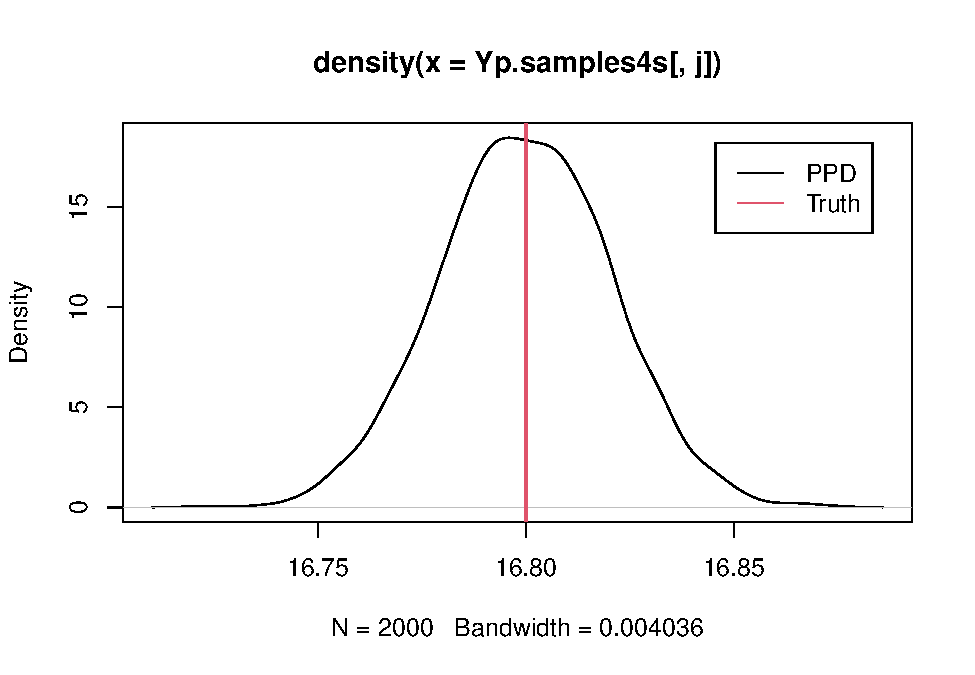
\includegraphics{st440hw5_files/figure-latex/unnamed-chunk-14-1.pdf}
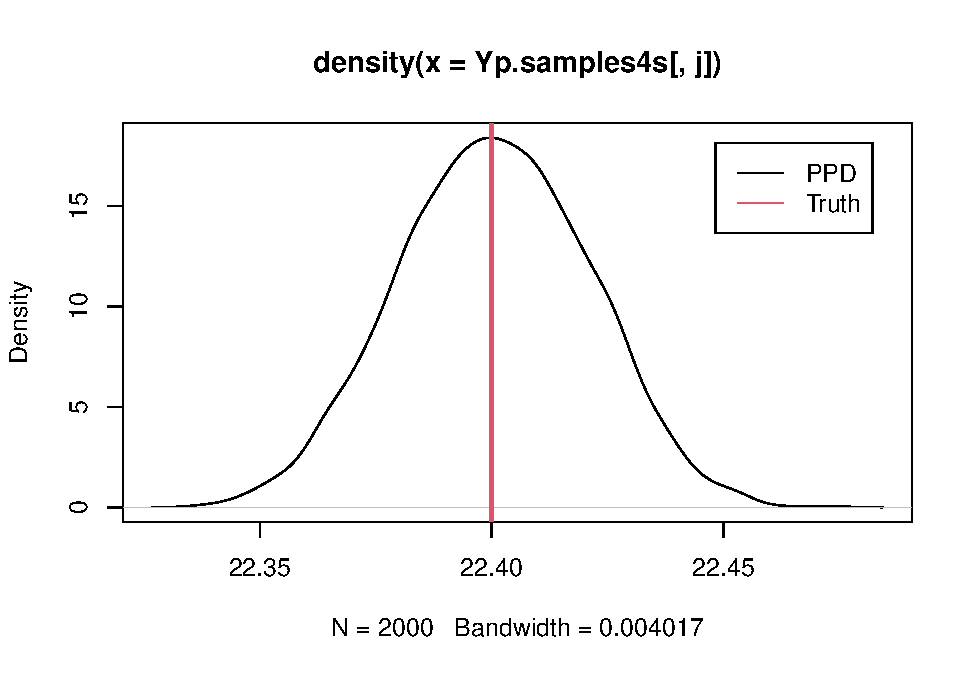
\includegraphics{st440hw5_files/figure-latex/unnamed-chunk-14-2.pdf}
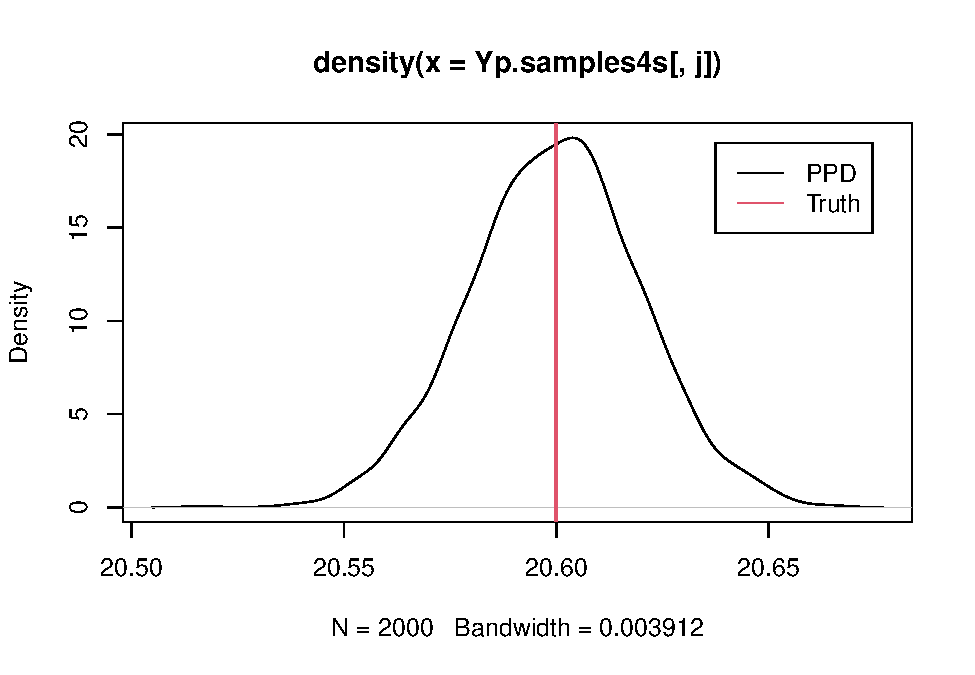
\includegraphics{st440hw5_files/figure-latex/unnamed-chunk-14-3.pdf}
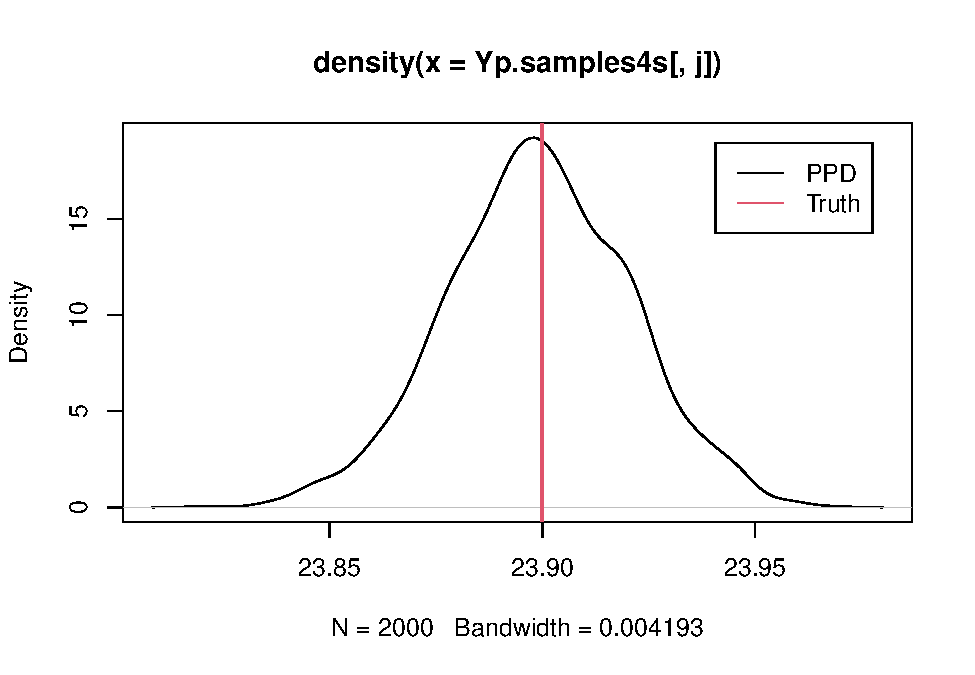
\includegraphics{st440hw5_files/figure-latex/unnamed-chunk-14-4.pdf}
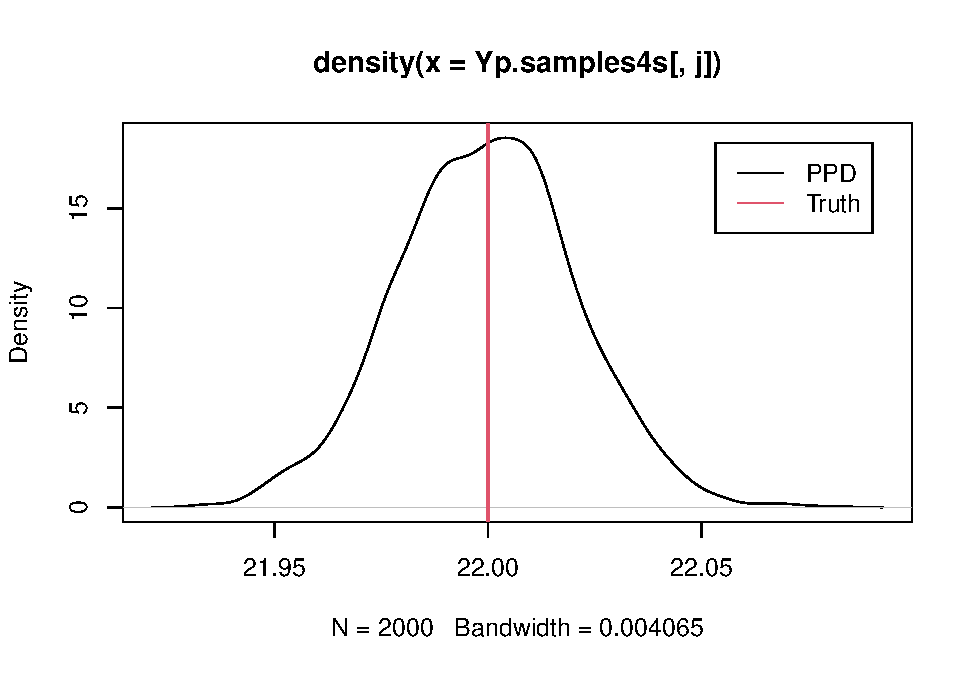
\includegraphics{st440hw5_files/figure-latex/unnamed-chunk-14-5.pdf}
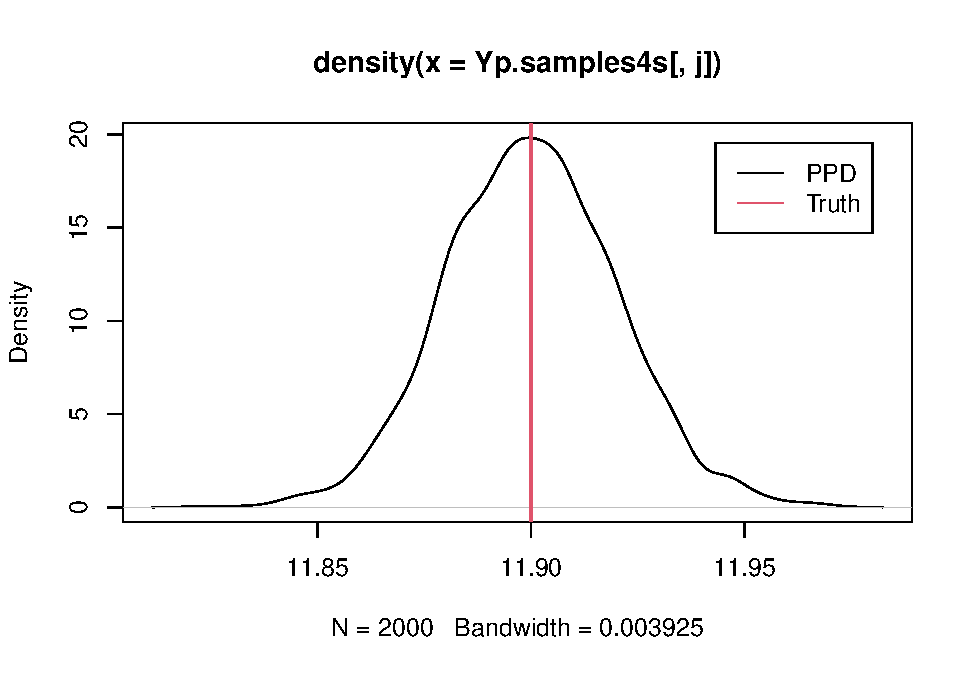
\includegraphics{st440hw5_files/figure-latex/unnamed-chunk-14-6.pdf}
Looks reasonable as the peak of the densities are around of the abline
of the true values.

\end{document}
